
%% bare_conf.tex
%% V1.3
%% 2007/01/11
%% by Michael Shell
%% See:
%% http://www.michaelshell.org/
%% for current contact information.
%%
%% This is a skeleton file demonstrating the use of IEEEtran.cls
%% (requires IEEEtran.cls version 1.7 or later) with an IEEE conference paper.
%%
%% Support sites:
%% http://www.michaelshell.org/tex/ieeetran/
%% http://www.ctan.org/tex-archive/macros/latex/contrib/IEEEtran/
%% and
%% http://www.ieee.org/

%%*************************************************************************
%% Legal Notice:
%% This code is offered as-is without any warranty either expressed or
%% implied; without even the implied warranty of MERCHANTABILITY or
%% FITNESS FOR A PARTICULAR PURPOSE! 
%% User assumes all risk.
%% In no event shall IEEE or any contributor to this code be liable for
%% any damages or losses, including, but not limited to, incidental,
%% consequential, or any other damages, resulting from the use or misuse
%% of any information contained here.
%%
%% All comments are the opinions of their respective authors and are not
%% necessarily endorsed by the IEEE.
%%
%% This work is distributed under the LaTeX Project Public License (LPPL)
%% ( http://www.latex-project.org/ ) version 1.3, and may be freely used,
%% distributed and modified. A copy of the LPPL, version 1.3, is included
%% in the base LaTeX documentation of all distributions of LaTeX released
%% 2003/12/01 or later.
%% Retain all contribution notices and credits.
%% ** Modified files should be clearly indicated as such, including  **
%% ** renaming them and changing author support contact information. **
%%
%% File list of work: IEEEtran.cls, IEEEtran_HOWTO.pdf, bare_adv.tex,
%%                    bare_conf.tex, bare_jrnl.tex, bare_jrnl_compsoc.tex
%%*************************************************************************

% *** Authors should verify (and, if needed, correct) their LaTeX system  ***
% *** with the testflow diagnostic prior to trusting their LaTeX platform ***
% *** with production work. IEEE's font choices can trigger bugs that do  ***
% *** not appear when using other class files.                            ***
% The testflow support page is at:
% http://www.michaelshell.org/tex/testflow/



% Note that the a4paper option is mainly intended so that authors in
% countries using A4 can easily print to A4 and see how their papers will
% look in print - the typesetting of the document will not typically be
% affected with changes in paper size (but the bottom and side margins will).
% Use the testflow package mentioned above to verify correct handling of
% both paper sizes by the user's LaTeX system.
%
% Also note that the "draftcls" or "draftclsnofoot", not "draft", option
% should be used if it is desired that the figures are to be displayed in
% draft mode.
%
\documentclass[conference]{IEEEtran}
% Add the compsoc option for Computer Society conferences.
%
% If IEEEtran.cls has not been installed into the LaTeX system files,
% manually specify the path to it like:
% \documentclass[conference]{../sty/IEEEtran}





% Some very useful LaTeX packages include:
% (uncomment the ones you want to load)


% *** MISC UTILITY PACKAGES ***
%
%\usepackage{ifpdf}
% Heiko Oberdiek's ifpdf.sty is very useful if you need conditional
% compilation based on whether the output is pdf or dvi.
% usage:
% \ifpdf
%   % pdf code
% \else
%   % dvi code
% \fi
% The latest version of ifpdf.sty can be obtained from:
% http://www.ctan.org/tex-archive/macros/latex/contrib/oberdiek/
% Also, note that IEEEtran.cls V1.7 and later provides a builtin
% \ifCLASSINFOpdf conditional that works the same way.
% When switching from latex to pdflatex and vice-versa, the compiler may
% have to be run twice to clear warning/error messages.






% *** CITATION PACKAGES ***
%
%\usepackage{cite}
% cite.sty was written by Donald Arseneau
% V1.6 and later of IEEEtran pre-defines the format of the cite.sty package
% \cite{} output to follow that of IEEE. Loading the cite package will
% result in citation numbers being automatically sorted and properly
% "compressed/ranged". e.g., [1], [9], [2], [7], [5], [6] without using
% cite.sty will become [1], [2], [5]--[7], [9] using cite.sty. cite.sty's
% \cite will automatically add leading space, if needed. Use cite.sty's
% noadjust option (cite.sty V3.8 and later) if you want to turn this off.
% cite.sty is already installed on most LaTeX systems. Be sure and use
% version 4.0 (2003-05-27) and later if using hyperref.sty. cite.sty does
% not currently provide for hyperlinked citations.
% The latest version can be obtained at:
% http://www.ctan.org/tex-archive/macros/latex/contrib/cite/
% The documentation is contained in the cite.sty file itself.






% *** GRAPHICS RELATED PACKAGES ***
%
\ifCLASSINFOpdf
  % \usepackage[pdftex]{graphicx}
  % declare the path(s) where your graphic files are
  % \graphicspath{{../pdf/}{../jpeg/}}
  % and their extensions so you won't have to specify these with
  % every instance of \includegraphics
  % \DeclareGraphicsExtensions{.pdf,.jpeg,.png}
\else
  % or other class option (dvipsone, dvipdf, if not using dvips). graphicx
  % will default to the driver specified in the system graphics.cfg if no
  % driver is specified.
  % \usepackage[dvips]{graphicx}
  % declare the path(s) where your graphic files are
  % \graphicspath{{../eps/}}
  % and their extensions so you won't have to specify these with
  % every instance of \includegraphics
  % \DeclareGraphicsExtensions{.eps}
\fi
% graphicx was written by David Carlisle and Sebastian Rahtz. It is
% required if you want graphics, photos, etc. graphicx.sty is already
% installed on most LaTeX systems. The latest version and documentation can
% be obtained at: 
% http://www.ctan.org/tex-archive/macros/latex/required/graphics/
% Another good source of documentation is "Using Imported Graphics in
% LaTeX2e" by Keith Reckdahl which can be found as epslatex.ps or
% epslatex.pdf at: http://www.ctan.org/tex-archive/info/
%
% latex, and pdflatex in dvi mode, support graphics in encapsulated
% postscript (.eps) format. pdflatex in pdf mode supports graphics
% in .pdf, .jpeg, .png and .mps (metapost) formats. Users should ensure
% that all non-photo figures use a vector format (.eps, .pdf, .mps) and
% not a bitmapped formats (.jpeg, .png). IEEE frowns on bitmapped formats
% which can result in "jaggedy"/blurry rendering of lines and letters as
% well as large increases in file sizes.
%
% You can find documentation about the pdfTeX application at:
% http://www.tug.org/applications/pdftex





% *** MATH PACKAGES ***
%
%\usepackage[cmex10]{amsmath}
% A popular package from the American Mathematical Society that provides
% many useful and powerful commands for dealing with mathematics. If using
% it, be sure to load this package with the cmex10 option to ensure that
% only type 1 fonts will utilized at all point sizes. Without this option,
% it is possible that some math symbols, particularly those within
% footnotes, will be rendered in bitmap form which will result in a
% document that can not be IEEE Xplore compliant!
%
% Also, note that the amsmath package sets \interdisplaylinepenalty to 10000
% thus preventing page breaks from occurring within multiline equations. Use:
%\interdisplaylinepenalty=2500
% after loading amsmath to restore such page breaks as IEEEtran.cls normally
% does. amsmath.sty is already installed on most LaTeX systems. The latest
% version and documentation can be obtained at:
% http://www.ctan.org/tex-archive/macros/latex/required/amslatex/math/





% *** SPECIALIZED LIST PACKAGES ***
%
%\usepackage{algorithmic}
% algorithmic.sty was written by Peter Williams and Rogerio Brito.
% This package provides an algorithmic environment fo describing algorithms.
% You can use the algorithmic environment in-text or within a figure
% environment to provide for a floating algorithm. Do NOT use the algorithm
% floating environment provided by algorithm.sty (by the same authors) or
% algorithm2e.sty (by Christophe Fiorio) as IEEE does not use dedicated
% algorithm float types and packages that provide these will not provide
% correct IEEE style captions. The latest version and documentation of
% algorithmic.sty can be obtained at:
% http://www.ctan.org/tex-archive/macros/latex/contrib/algorithms/
% There is also a support site at:
% http://algorithms.berlios.de/index.html
% Also of interest may be the (relatively newer and more customizable)
% algorithmicx.sty package by Szasz Janos:
% http://www.ctan.org/tex-archive/macros/latex/contrib/algorithmicx/




% *** ALIGNMENT PACKAGES ***
%
%\usepackage{array}
% Frank Mittelbach's and David Carlisle's array.sty patches and improves
% the standard LaTeX2e array and tabular environments to provide better
% appearance and additional user controls. As the default LaTeX2e table
% generation code is lacking to the point of almost being broken with
% respect to the quality of the end results, all users are strongly
% advised to use an enhanced (at the very least that provided by array.sty)
% set of table tools. array.sty is already installed on most systems. The
% latest version and documentation can be obtained at:
% http://www.ctan.org/tex-archive/macros/latex/required/tools/


%\usepackage{mdwmath}
%\usepackage{mdwtab}
% Also highly recommended is Mark Wooding's extremely powerful MDW tools,
% especially mdwmath.sty and mdwtab.sty which are used to format equations
% and tables, respectively. The MDWtools set is already installed on most
% LaTeX systems. The lastest version and documentation is available at:
% http://www.ctan.org/tex-archive/macros/latex/contrib/mdwtools/


% IEEEtran contains the IEEEeqnarray family of commands that can be used to
% generate multiline equations as well as matrices, tables, etc., of high
% quality.


%\usepackage{eqparbox}
% Also of notable interest is Scott Pakin's eqparbox package for creating
% (automatically sized) equal width boxes - aka "natural width parboxes".
% Available at:
% http://www.ctan.org/tex-archive/macros/latex/contrib/eqparbox/





% *** SUBFIGURE PACKAGES ***
%\usepackage[tight,footnotesize]{subfigure}
% subfigure.sty was written by Steven Douglas Cochran. This package makes it
% easy to put subfigures in your figures. e.g., "Figure 1a and 1b". For IEEE
% work, it is a good idea to load it with the tight package option to reduce
% the amount of white space around the subfigures. subfigure.sty is already
% installed on most LaTeX systems. The latest version and documentation can
% be obtained at:
% http://www.ctan.org/tex-archive/obsolete/macros/latex/contrib/subfigure/
% subfigure.sty has been superceeded by subfig.sty.



%\usepackage[caption=false]{caption}
%\usepackage[font=footnotesize]{subfig}
% subfig.sty, also written by Steven Douglas Cochran, is the modern
% replacement for subfigure.sty. However, subfig.sty requires and
% automatically loads Axel Sommerfeldt's caption.sty which will override
% IEEEtran.cls handling of captions and this will result in nonIEEE style
% figure/table captions. To prevent this problem, be sure and preload
% caption.sty with its "caption=false" package option. This is will preserve
% IEEEtran.cls handing of captions. Version 1.3 (2005/06/28) and later 
% (recommended due to many improvements over 1.2) of subfig.sty supports
% the caption=false option directly:
%\usepackage[caption=false,font=footnotesize]{subfig}
%
% The latest version and documentation can be obtained at:
% http://www.ctan.org/tex-archive/macros/latex/contrib/subfig/
% The latest version and documentation of caption.sty can be obtained at:
% http://www.ctan.org/tex-archive/macros/latex/contrib/caption/




% *** FLOAT PACKAGES ***
%
%\usepackage{fixltx2e}
% fixltx2e, the successor to the earlier fix2col.sty, was written by
% Frank Mittelbach and David Carlisle. This package corrects a few problems
% in the LaTeX2e kernel, the most notable of which is that in current
% LaTeX2e releases, the ordering of single and double column floats is not
% guaranteed to be preserved. Thus, an unpatched LaTeX2e can allow a
% single column figure to be placed prior to an earlier double column
% figure. The latest version and documentation can be found at:
% http://www.ctan.org/tex-archive/macros/latex/base/



%\usepackage{stfloats}
% stfloats.sty was written by Sigitas Tolusis. This package gives LaTeX2e
% the ability to do double column floats at the bottom of the page as well
% as the top. (e.g., "\begin{figure*}[!b]" is not normally possible in
% LaTeX2e). It also provides a command:
%\fnbelowfloat
% to enable the placement of footnotes below bottom floats (the standard
% LaTeX2e kernel puts them above bottom floats). This is an invasive package
% which rewrites many portions of the LaTeX2e float routines. It may not work
% with other packages that modify the LaTeX2e float routines. The latest
% version and documentation can be obtained at:
% http://www.ctan.org/tex-archive/macros/latex/contrib/sttools/
% Documentation is contained in the stfloats.sty comments as well as in the
% presfull.pdf file. Do not use the stfloats baselinefloat ability as IEEE
% does not allow \baselineskip to stretch. Authors submitting work to the
% IEEE should note that IEEE rarely uses double column equations and
% that authors should try to avoid such use. Do not be tempted to use the
% cuted.sty or midfloat.sty packages (also by Sigitas Tolusis) as IEEE does
% not format its papers in such ways.





% *** PDF, URL AND HYPERLINK PACKAGES ***
%
%\usepackage{url}
% url.sty was written by Donald Arseneau. It provides better support for
% handling and breaking URLs. url.sty is already installed on most LaTeX
% systems. The latest version can be obtained at:
% http://www.ctan.org/tex-archive/macros/latex/contrib/misc/
% Read the url.sty source comments for usage information. Basically,
% \url{my_url_here}.





% *** Do not adjust lengths that control margins, column widths, etc. ***
% *** Do not use packages that alter fonts (such as pslatex).         ***
% There should be no need to do such things with IEEEtran.cls V1.6 and later.
% (Unless specifically asked to do so by the journal or conference you plan
% to submit to, of course. )

\usepackage{graphicx}
\usepackage{subfigure}
\usepackage[justification=centering]{caption}

% correct bad hyphenation here
\hyphenation{op-tical net-works semi-conduc-tor}


\begin{document}
%
% paper title
% can use linebreaks \\ within to get better formatting as desired
\title{Automatic object detection and segmentation from underwater images via saliency-based region merging}


% author names and affiliations
% use a multiple column layout for up to three different
% affiliations
\author{\IEEEauthorblockN{Yafei Zhu, Xinxin Qiu, Xiaoqing Sun, Haiyong Zheng$^{\ast}$, Bing Zheng}
\IEEEauthorblockA{Department of Electronic Engineering\\
College of Information Science and Engineering\\
Ocean University of China\\
$^{\ast}$Corresponding author: zhenghaiyong@ouc.edu.cn}}
%\and
%\IEEEauthorblockN{Homer Simpson}
%\IEEEauthorblockA{Twentieth Century Fox\\
%Springfield, USA\\
%Email: homer@thesimpsons.com}
%\and
%\IEEEauthorblockN{James Kirk\\ and Montgomery Scott}
%\IEEEauthorblockA{Starfleet Academy\\
%San Francisco, California 96678-2391\\
%Telephone: (800) 555--1212\\
%Fax: (888) 555--1212}}

% conference papers do not typically use \thanks and this command
% is locked out in conference mode. If really needed, such as for
% the acknowledgment of grants, issue a \IEEEoverridecommandlockouts
% after \documentclass

% for over three affiliations, or if they all won't fit within the width
% of the page, use this alternative format:
% 
%\author{\IEEEauthorblockN{Michael Shell\IEEEauthorrefmark{1},
%Homer Simpson\IEEEauthorrefmark{2},
%James Kirk\IEEEauthorrefmark{3}, 
%Montgomery Scott\IEEEauthorrefmark{3} and
%Eldon Tyrell\IEEEauthorrefmark{4}}
%\IEEEauthorblockA{\IEEEauthorrefmark{1}School of Electrical and Computer Engineering\\
%Georgia Institute of Technology,
%Atlanta, Georgia 30332--0250\\ Email: see http://www.michaelshell.org/contact.html}
%\IEEEauthorblockA{\IEEEauthorrefmark{2}Twentieth Century Fox, Springfield, USA\\
%Email: homer@thesimpsons.com}
%\IEEEauthorblockA{\IEEEauthorrefmark{3}Starfleet Academy, San Francisco, California 96678-2391\\
%Telephone: (800) 555--1212, Fax: (888) 555--1212}
%\IEEEauthorblockA{\IEEEauthorrefmark{4}Tyrell Inc., 123 Replicant Street, Los Angeles, California 90210--4321}}




% use for special paper notices
%\IEEEspecialpapernotice{(Invited Paper)}




% make the title area
\maketitle


\begin{abstract}
%\boldmath
Underwater object detection and segmentation has been attracting a lot of interest, and recently various systems have been designed. In this paper, we introduce a novel technique to automatically detect and segment objects from underwater images via saliency-based region merging. The method is composed of three main steps. Firstly, a salient object detection model is used to detect the position of salient objects in underwater image. Secondly, background prior is applied to determine the approximate background location. Thirdly,  the region merging based interactive image segmentation method is improved by adding the determined object and background location information as the user inputs so that the algorithm becomes automatic. The experimental results show that it's efficient to segment objects from the underwater image by the proposed method.
%Our main idea is to use the salient object detection model (DRFI) to detect the position of salient objects in underwater image, then we improve the region merging based interactive image segmentation method (called MSRM) by adding the determined object information as the user inputs so that the algorithm becomes automatic. 
\end{abstract}
% IEEEtran.cls defaults to using nonbold math in the Abstract.
% This preserves the distinction between vectors and scalars. However,
% if the conference you are submitting to favors bold math in the abstract,
% then you can use LaTeX's standard command \boldmath at the very start
% of the abstract to achieve this. Many IEEE journals/conferences frown on
% math in the abstract anyway.

% no keywords




% For peer review papers, you can put extra information on the cover
% page as needed:
% \ifCLASSOPTIONpeerreview
% \begin{center} \bfseries EDICS Category: 3-BBND \end{center}
% \fi
%
% For peerreview papers, this IEEEtran command inserts a page break and
% creates the second title. It will be ignored for other modes.
\IEEEpeerreviewmaketitle



\section{Introduction}
% no \IEEEPARstart
%Underwater object detection and segmentation is critical in a lot of applications in maintenance, repair of undersea structures, marine sciences, and homeland security. However, the underwater images present some particular difficulties including natural and artificial illumination, color alteration, light attenuation [5], and marine snow.

%Object detection and segmentation from underwater images play an essential role in automatic tracking and recognition of underwater targets such as fishes. 

Recent years have witnessed rapidly increasing interest in underwater object detection and segmentation. It is motivated by the importance of underwater object detection and segmentation in applications such as in maintenance, repair of undersea structures, marine sciences, and homeland security.

%The purpose of image segmentation is to separate foreground objects from the image 

%Underwater object detection and segmentation has become more and more popular in recent years, 
Several underwater object detection and segmentation systems have been designed successfully. Kabatek et al.~\cite{kabatek2009underwater} did the research on underwater objects detection for electro-optical imagery data. Williams et al. presented a method for underwater target detection using context in ~\cite{williams2010using}. Shen et al.~\cite{shen2014biological} realized a successful system of moving object detection. An underwater acoustic image segmentation is proposed based on deformable template~\cite{sang2005underwater}. In~\cite{singh2014segmentation}, an efficient and fast underwater image segmentation method using thresholding with class 3 fuzzy C-means clustering and CLAHE enhancement method was proposed.

These methods have their own advantages and disadvantages, and none of them works equally well for all kinds of images. It is difficult to detect and segment objects in underwater environment without the details of the objects. Also, in the underwater object detection task, the decayed color and the haze effect would significantly decrease the contrast between the object and the background. Many traditional object detection methods are distorted and can hardly be taken for precise object detection.

After a long period of evolution, research on saliency detection has developed greatly. In salient object detection task, we only focus on the most salient objects in images. Though the underwater image is blurry and low contrast, we can still detect the position of relatively salient objects using salient object detection method. The leading method of all the benchmark salient object detection and segmentation methods in~\cite{borji2015salient} is a discriminative regional feature integration (DRFI) approach~\cite{jiang2013salient}. Instead of purely relying on the cues extracted only from the input image, DRFI resorts to human annotations to automatically discover feature integration rules, thus is more effective in detecting underwater objects than existing models.

The background prior, which assumes that the area in the narrow border of the image belongs to the background, performs very robust in many detection tasks. So we use background prior to determine the background location information in underwater images. 

Recently, semi-automatic segmentation techniques that allow solving moderate and hard segmentation tasks via user inputs are becoming more and more popular. Since object information can be obtained by salient object detection method and background information can be extracted by background prior, the semi-automatic segmentation method can then be improved to be automatic using the determined object and background location information instead of user inputs.

%However, the objects in underwater images are not clearly visible due to low contrast and high noise in the environment, which increases the difficulty of detection and segmentation. 

%For detecting and segmenting objects in underwater images, generally, a preprocessing step is applied to enhance the images. 
%The method must tackle these problems and is developed under two constraints: no human intervention, low processing time. For segmenting an object in an image, we first need to detect the presence of the object. The method is composed of two main steps:
%\begin{itemize}
%\item Detect the position of salient objects in underwater image
%\item Separate foreground objects from the image
%\end{itemize}



%To solve the above problems,  an image processing strategy strategy detect and segment the underwater object automatically is presented. 

The framework of our proposed method is shown in Fig.~\ref{fig:flowchart}. Firstly, the dark channel prior~\cite{he2011single} is applied to enhance the image by removing the ``haze'' that makes the underwater image unclear. Then, for detecting salient objects in the enhanced image with complicated background, we choose DRFI~\cite{jiang2013salient} model to generate the saliency map containing ``saliency values'' per pixel. And the obtained saliency map is further processed to determine the location information of object and background. Finally, the maximal similarity based region merging (MSRM) method~\cite{ning2010interactive} is improved to be automatic by adding the determined object and background location information as the user inputs. 

\begin{figure*}[t]
\centerline{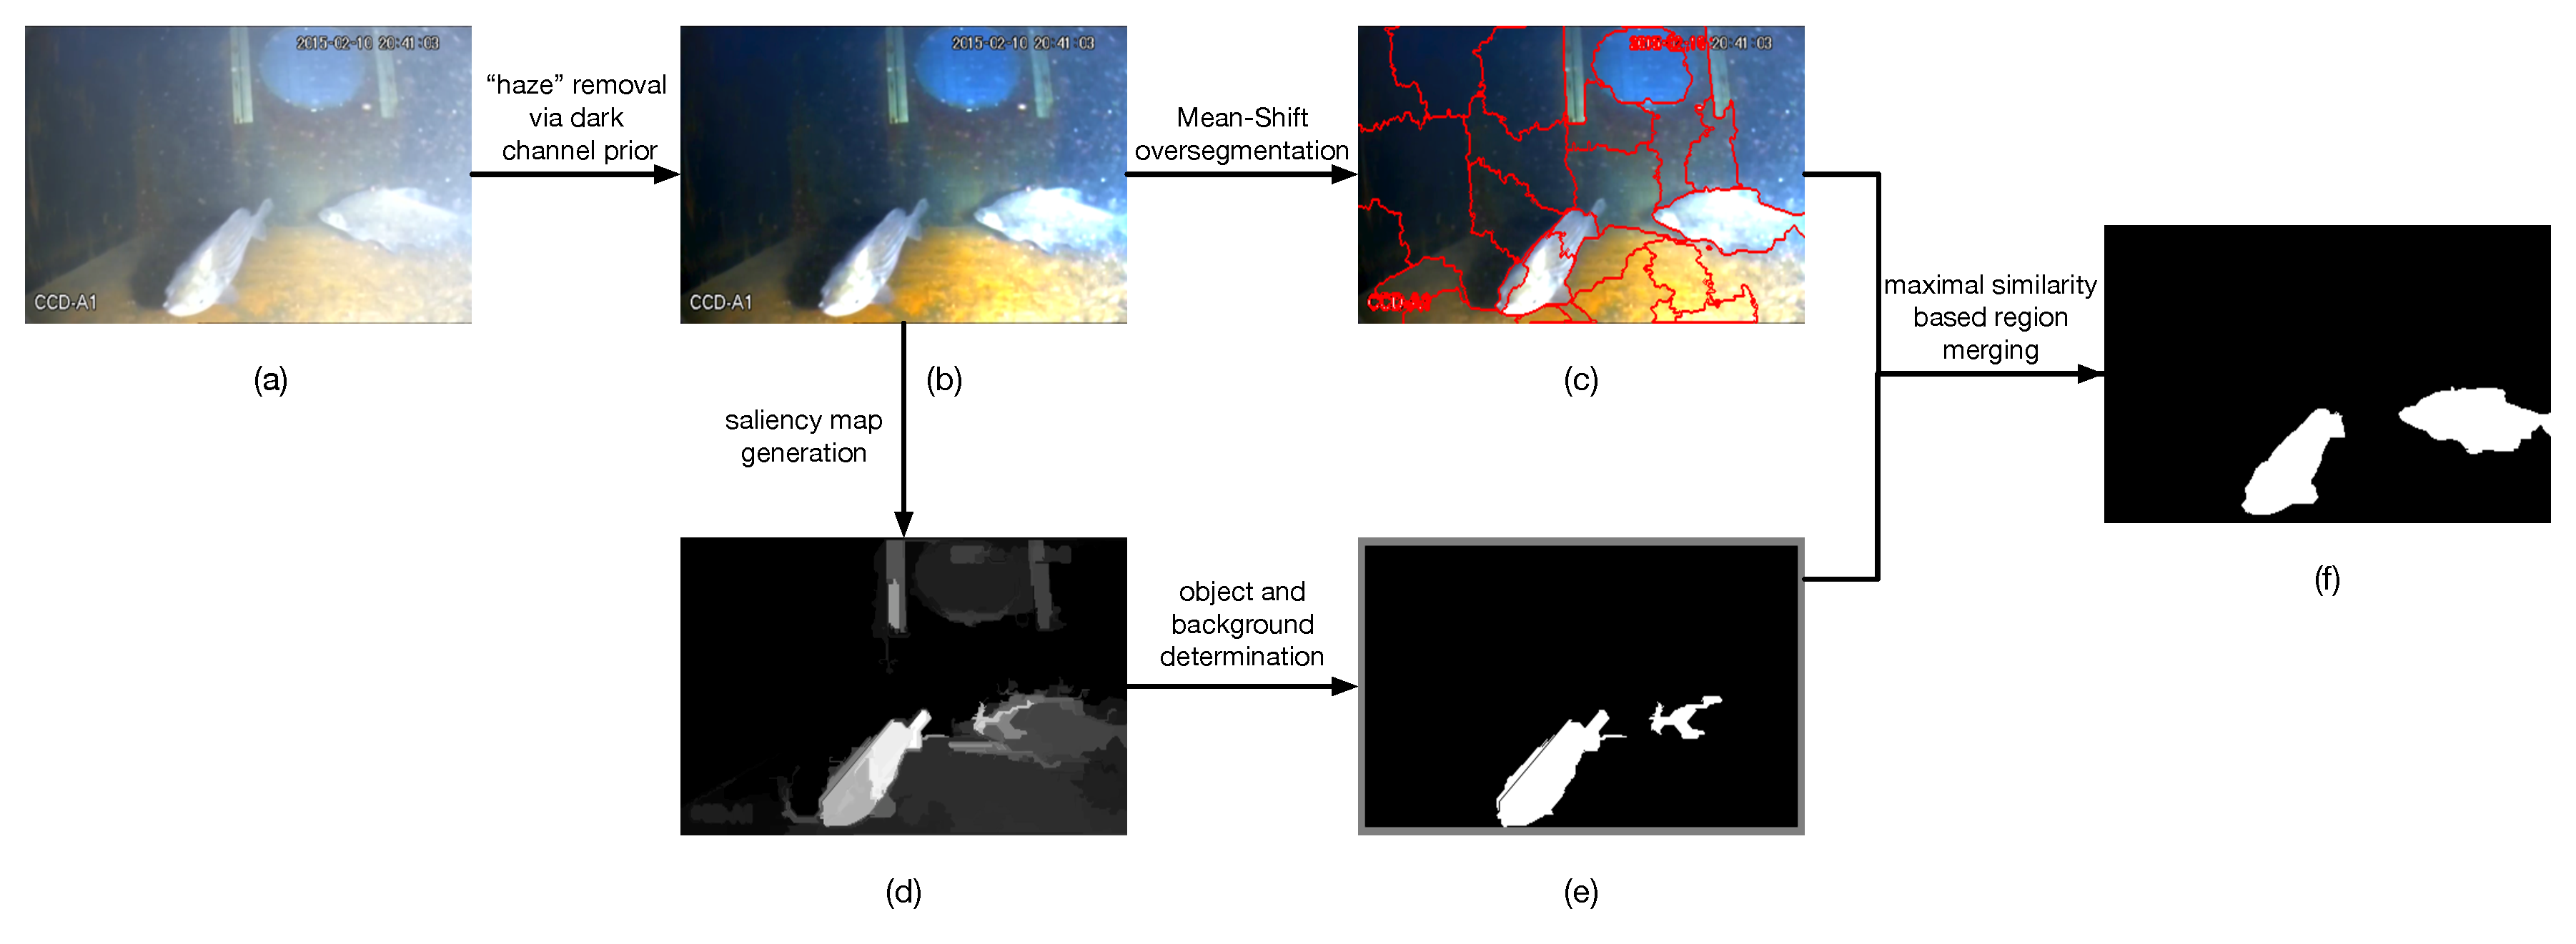
\includegraphics[width=\textwidth]{figures/flowchart.eps}}
\caption{The framework of our proposed method for object detection and segmentation from underwater images.}
\label{fig:flowchart}
\end{figure*} 

\section{Method}

\subsection{Dark channel prior algorithm}
The dark channel prior was proposed to remove haze from a single input image~\cite{he2011single}. It is based on the following observation on haze-free outdoor images: in most of the non-sky patches, at least one color channel has very low intensity at some pixels. In other words, the minimum intensity in such a patch should has a very low value. Formally, for an image $\mathbf{J}$, its dark channel is defined as
\begin{equation}
J^{dark}(x) = \min_{c\in \{r,g,b\}}(\min_{y\in \Omega(x)}(J^c(y)))
\end{equation}
where $J^c$ is a color channel of $\mathbf{J}$ and $\Omega(x)$ is a local patch centered at x. Except for the sky region, the intensity of $J^{dark}$ is low and tends to be zero, if \textbf{J} is a haze-free outdoor image. And the above statistical observation or knowledge is called the \textit{dark channel prior}.

In computer vision and computer graphics, the model widely used to describe the formation of a haze image is as follows:
\begin{equation}
\mathbf{I}(x) = \mathbf{J}(x)t(x) + \mathbf{A}(1 - t(x))
\label{Eq: HazeImaging}
\end{equation}
where $\mathbf{I}$ is the observed intensity, $\mathbf{J}$ is the scene radiance, $\mathbf{A}$ is the global atmospheric light, and $t$ is the medium trans- mission describing the portion of the light that is not scat- tered and reaches the camera. The goal of haze removal is to recover $\mathbf{J}$, $\mathbf{A}$, and $t$ from $\mathbf{I}$.

Using the haze imaging Equation (\ref{Eq: HazeImaging}) and the dark channel prior together, the final scene radiance $\mathbf{J}(x)$ can be derived as:
\begin{equation}
\mathbf{J}(x) = \frac{\mathbf{I}(x)-\mathbf{A}}{max(t(x), t_0)} + \mathbf{A}
\end{equation}
A typical value of $t_0$ is 0.1.

The dark channel prior is effective for a variety of hazy images while it maybe invalid when the scene objects are inherently similar to the atmospheric light and no shadow is cast on them.

The underwater images are similar with the haze images as they are all degraded by medium. Besides, they doesn't conform the failure condition. Therefore, dark channel prior algorithm can be used to remove the ‘haze’ in underwater images. Fig.~\ref{fig:flowchart}(b) shows an example of the result processed by the dark channel prior. 

\begin{figure*}[!t]
  \centering 
  \subfigure[]{ 
    \label{fig:comparison:a} %% label for first subfigure 
    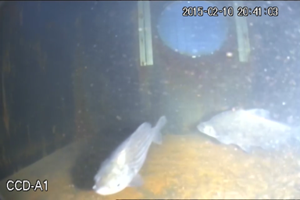
\includegraphics[width=0.3\textwidth]{figures/originalImage.png}} 
  \subfigure[]{ 
    \label{fig:comparison:b} %% label for first subfigure 
    
\includegraphics[width=0.3\textwidth]{figures/segmentationResult.png}} 
  \subfigure[]{ 
    \label{fig:comparison:c} %% label for second subfigure 
    
\includegraphics[width=0.3\textwidth]{figures/groundTruth.png}} 
    
  \subfigure[]{ 
    \label{fig:comparison:a} %% label for first subfigure 
    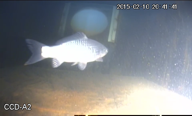
\includegraphics[width=0.3\textwidth]{figures/originalImage1.png}} 
  \subfigure[]{ 
    \label{fig:comparison:b} %% label for first subfigure 
    
\includegraphics[width=0.3\textwidth]{figures/segmentationResult1.png}} 
  \subfigure[]{ 
    \label{fig:comparison:c} %% label for second subfigure 
    
\includegraphics[width=0.3\textwidth]{figures/groundTruth1.png}} 
    
    \subfigure[]{ 
    \label{fig:comparison:a} %% label for first subfigure 
    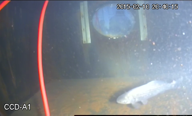
\includegraphics[width=0.3\textwidth]{figures/originalImage2.png}} 
  \subfigure[]{ 
    \label{fig:comparison:b} %% label for first subfigure 
    
\includegraphics[width=0.3\textwidth]{figures/segmentationResult2.png}} 
  \subfigure[]{ 
    \label{fig:comparison:c} %% label for second subfigure 
    
\includegraphics[width=0.3\textwidth]{figures/groundTruth2.png}} 
  \caption{Qualitative comparison: (a)(d)(g) Original image. (b)(e)(h) Our segmentation result. (c)(f)(i) Human labeled map.}
  \label{fig:comparison} %% label for entire figure 
\end{figure*}

\subsection{Discriminative Regional Feature Integration (DRFI) algorithm}

Salient object detection method can be used to approximately obtain the location of the foreground, in terms of saliency map, from an image where the foreground would draw the attentions of humans at the first sight of an image. In practice, salient object detection methods are commonly used as a first step of many applications including object recognition, object segmentation, object tracking and so on. Recently, a lot of research efforts have been made for saliency computation. A comprehensive survey of salient object detection can be found from~\cite{borji2014salientsurvey}.

Jiang et al.~\cite{jiang2013salient} address the salient object detection problem using a discriminative regional feature integration (DRFI) approach. It integrates the regional contrast, regional property and regional backgroundness descriptors together to form the master saliency map, thus can deal with the challenging cases such as detecting salient objects from low-quality underwater images. Fig.~\ref{fig:flowchart}(d) shows an example of saliency map generated by DRFI.

\subsection{Object and background determination}

For each pixel in the saliency map, the higher of the value, the more salient of it in the original image. In other words, normally, for an image, pixels which have higher values in the corresponding saliency map belong to objects. Therefore, pixels whose values in the saliency map are greater than a certain threshold can be taken as object pixels. The Otsu method~\cite{otsu1975threshold} is adopted to compute the threshold from the saliency map for the determination of object location information. 

The background prior assumes that the image boundary is mostly background, so we take pixels in the $6$-pixel wide narrow border region of the image as background pixels.

In Fig.~\ref{fig:flowchart}(e), we use marks to indicate the object and background location information. The white parts are the object markers while the gray parts in the image boundary are the background markers, the remaining black parts are non-marked. 

\subsection{Mean-Shift oversegmentation}

An initial segmentation is required to partition the image into homogeneous regions for merging. Any existing low level segmentation methods, such as mean shift~\cite{cheng1995mean,comaniciu2002mean}, watershed~\cite{vincent1991watersheds}, SLIC~\cite{achanta2012slic} and Turbopixel~\cite{levinshtein2009turbopixels}, can be used for this step. In this paper, we choose to use the mean shift method for initial segmentation because it has less over segmentation and can well preserve the object boundaries. Fig.~\ref{fig:flowchart}(c) shows an example of the mean shift initial segmentation.

\subsection{Object and background marking}

For each region in the oversegmented result (Fig.~\ref{fig:flowchart}(c)),  we regard it as background region (denoted by $M_B$) if there is at least one background pixel in it, then, a region is regarded as object region (denoted by $M_O$) if the number of object pixels in it accounts for more than 10\% of the region area. If there is neither object nor background pixel in one region, we call it non-marker region, denoted by $N$. Now the whole image is divided into three parts: $M_O$, $M_B$, and $N$.

\subsection{Maximal-similarity based region merging}

After mean shift initial segmentation, we have many small regions available. To guide the following region merging process, some descriptor for representing these regions and a rule for merging are needed.

\subsubsection{Region representation}

The initially segmented small regions of the desired object often vary a lot in size and shape, while the colors of different regions from the same object will have high similarity. Therefore, the color histogram is used to represent each region in this paper. We uniformly quantize each color channel into $16$ levels and then the histogram of each region is calculated in the feature space of $16\times16\times16 = 4096$ bins. Denote by $Hist_R$ the normalized histogram of a region $R$. 

\subsubsection{Similarity measure}

A similarity measure $\rho(R, Q)$ between two region $R$ and $Q$ is defined to accommodate the comparison between various regions. 
\begin{equation}
\rho(R, Q) = \sum_{u=1}^{4096}\sqrt{Hist_R^u\cdot Hist_Q^u}
\label{Eq: SimilarityMeasure}
\end{equation}

\subsubsection{Maximal similarity based merging rule}

Let $Q$ be an adjacent region of $R$ and denote by $\bar{S}_Q = \{S_i^Q\}_{i=1,2,\ldots,q}$ the set of $Q$'s adjacent regions. The similarity between $Q$ and all its adjacent regions, i.e. $\rho(Q, S_i^Q), i=1,2,\ldots,q$, are calculated. Obviously, $R$ is a member of $\bar{S}_Q$. If the similarity between $R$ and $Q$ is the maximal one among all the similarities $\rho(Q, S_i^Q)$, we will merge $R$ and $Q$. The following merging rule is defined:
\begin{equation}
\mbox{Merge $R$ and $Q$ \quad if } \rho(R, Q) = \max_{i=1,2,\ldots,q}\rho(Q, S_i^Q)
\label{Eq: MergingRule}
\end{equation}

\subsubsection{The merging process}

The whole region merging process can be divided into two stages. In the first stage, merging non-marker regions in $N$ with marker background regions in $M_B$. In the second stage, merging non-marker regions in $N$ adaptively. Fig.~\ref{fig:flowchart}(f) shows an example of the final segmentation result after region merging.



%\subsubsection{Subsubsection Heading Here}
%Subsubsection text here.


% An example of a floating figure using the graphicx package.
% Note that \label must occur AFTER (or within) \caption.
% For figures, \caption should occur after the \includegraphics.
% Note that IEEEtran v1.7 and later has special internal code that
% is designed to preserve the operation of \label within \caption
% even when the captionsoff option is in effect. However, because
% of issues like this, it may be the safest practice to put all your
% \label just after \caption rather than within \caption{}.
%
% Reminder: the "draftcls" or "draftclsnofoot", not "draft", class
% option should be used if it is desired that the figures are to be
% displayed while in draft mode.
%
%\begin{figure}[!t]
%\centering
%\includegraphics[width=2.5in]{myfigure}
% where an .eps filename suffix will be assumed under latex, 
% and a .pdf suffix will be assumed for pdflatex; or what has been declared
% via \DeclareGraphicsExtensions.
%\caption{Simulation Results}
%\label{fig_sim}
%\end{figure}

% Note that IEEE typically puts floats only at the top, even when this
% results in a large percentage of a column being occupied by floats.


% An example of a double column floating figure using two subfigures.
% (The subfig.sty package must be loaded for this to work.)
% The subfigure \label commands are set within each subfloat command, the
% \label for the overall figure must come after \caption.
% \hfil must be used as a separator to get equal spacing.
% The subfigure.sty package works much the same way, except \subfigure is
% used instead of \subfloat.
%
%\begin{figure*}[!t]
%\centerline{\subfloat[Case I]\includegraphics[width=2.5in]{subfigcase1}%
%\label{fig_first_case}}
%\hfil
%\subfloat[Case II]{\includegraphics[width=2.5in]{subfigcase2}%
%\label{fig_second_case}}}
%\caption{Simulation results}
%\label{fig_sim}
%\end{figure*}
%
% Note that often IEEE papers with subfigures do not employ subfigure
% captions (using the optional argument to \subfloat), but instead will
% reference/describe all of them (a), (b), etc., within the main caption.


% An example of a floating table. Note that, for IEEE style tables, the 
% \caption command should come BEFORE the table. Table text will default to
% \footnotesize as IEEE normally uses this smaller font for tables.
% The \label must come after \caption as always.
%
%\begin{table}[!t]
%% increase table row spacing, adjust to taste
%\renewcommand{\arraystretch}{1.3}
% if using array.sty, it might be a good idea to tweak the value of
% \extrarowheight as needed to properly center the text within the cells
%\caption{An Example of a Table}
%\label{table_example}
%\centering
%% Some packages, such as MDW tools, offer better commands for making tables
%% than the plain LaTeX2e tabular which is used here.
%\begin{tabular}{|c||c|}
%\hline
%One & Two\\
%\hline
%Three & Four\\
%\hline
%\end{tabular}
%\end{table}


% Note that IEEE does not put floats in the very first column - or typically
% anywhere on the first page for that matter. Also, in-text middle ("here")
% positioning is not used. Most IEEE journals/conferences use top floats
% exclusively. Note that, LaTeX2e, unlike IEEE journals/conferences, places
% footnotes above bottom floats. This can be corrected via the \fnbelowfloat
% command of the stfloats package.

\section{EXPERIMENTAL RESULTS}

Fig.~\ref{fig:comparison} shows three examples of the results: (a), (d) and (g) are original images captured from underwater videos, (b), (e) and (h) are the final segmentation results, while (c), (f) and (i) are ground truth labeled by human. 

As can be seen, (a) contains two objects, while (d) and (g) each contains one single object. The background in these images are all complex and have low contrast with the objects. From the segmentation results, we can see that our method can deal with the challenging cases where the background is cluttered and segment the right number of objects in all these images. Also, most meaningful object information can be extracted. However, it fails at some details such as the fish tail part in all these images, since the fish tail shares more commons with the underwater background both in color and luminance.

%The experimental results shows that most meaningful object information can be extracted through our method, which means it is effective for underwater object segmentation.

\section{Conclusion}
In this paper, we address the underwater object detection and segmentation problem using a saliency-based region merging approach. The success of our approach stems from three key factors. One is that we introduce salient object detection method to determine the spatial location of salient objects in blurry and miscolored underwater image. The second one is that we apply background prior to determine the background location information. The last one is that we integrate semi-automatic region merging framework and the object and background location information into a new automatic framework. The experimental results prove that the presented method is valid.


% conference papers do not normally have an appendix


% use section* for acknowledgement
\section*{Acknowledgment}

This work was supported by National Natural Science Foundation of China (Grant No. 61301240 and No. 61271406), Natural Science Foundation of Shandong Province (Grant No. ZR2014FQ027) and Basic Research Program of Qingdao Municipal Scientific Plan (Grant No. 13-1-4-223-jch).





% trigger a \newpage just before the given reference
% number - used to balance the columns on the last page
% adjust value as needed - may need to be readjusted if
% the document is modified later
%\IEEEtriggeratref{8}
% The "triggered" command can be changed if desired:
%\IEEEtriggercmd{\enlargethispage{-5in}}

% references section

% can use a bibliography generated by BibTeX as a .bbl file
% BibTeX documentation can be easily obtained at:
% http://www.ctan.org/tex-archive/biblio/bibtex/contrib/doc/
% The IEEEtran BibTeX style support page is at:
% http://www.michaelshell.org/tex/ieeetran/bibtex/
%\bibliographystyle{IEEEtran}
% argument is your BibTeX string definitions and bibliography database(s)
%\bibliography{IEEEabrv,../bib/paper}
%
% <OR> manually copy in the resultant .bbl file
% set second argument of \begin to the number of references
% (used to reserve space for the reference number labels box)
%\begin{thebibliography}{1}
%
%\bibitem{IEEEhowto:kopka}
%H.~Kopka and P.~W. Daly, \emph{A Guide to \LaTeX}, 3rd~ed.\hskip 1em plus
%  0.5em minus 0.4em\relax Harlow, England: Addison-Wesley, 1999.
%
%\end{thebibliography}

\bibliographystyle{IEEEtran}
\bibliography{IEEEabrv,bare_conf}

% that's all folks
\end{document}


